\chapter{Combustion: Fuels, Products and Greenhouse Gases}\label{ch:g8:combustion-and-fuels}

A family sleeps in a flat whose gas boiler has a blocked flue. The flame,
starved of \omterm{def:g4:air-a-mixture-of-gases:air}{air}, burns badly, and an invisible gas with no smell slowly
fills the rooms. At two in the morning a small box on the wall starts to
shriek: the carbon monoxide alarm. Everyone gets out in time. The same
\omterm{def:g4:what-a-fire-needs:fuel}{fuel}, \omterm{def:g4:what-a-fire-needs:burning}{burning} well, gives only carbon dioxide and water --- and that
carbon dioxide has its own story, written in the \omterm{def:g4:air-a-mixture-of-gases:air}{air} of the whole
planet.

\begin{recall}
A \omterm{def:g4:what-a-fire-needs:burning}{burning}, or \omterm{def:g4:what-a-fire-needs:burning}{combustion}, needs a \omterm{def:g4:what-a-fire-needs:fuel}{fuel}, oxygen and heat, and makes new
substances (\cref{ch:g4:what-a-fire-needs}). \omterm{def:g4:air-a-mixture-of-gases:air}{Air} is about one fifth
oxygen (\cref{ch:g4:air-a-mixture-of-gases}). An equation is balanced
when each kind of \omterm{def:g7:atoms-and-molecules:atom}{atom} appears the same number of times on both sides
(\cref{ch:g8:balanced-equations}).
\end{recall}

\section{Burning carbon and methane}

\begin{example}[Two combustions]\label{ex:g8:combustion-and-fuels:two}
Carbon (charcoal, coal) burns to give carbon dioxide:
\[
  \ce{C(s) + O2(g) -> CO2(g)}.
\]
Methane, the main part of natural gas, burns to give carbon dioxide and
water:
\[
  \ce{CH4(g) + 2O2(g) -> CO2(g) + 2H2O(l)}.
\]
In both cases limewater turns milky with the gas formed; with methane a
cold glass mists up as well.
\end{example}

\begin{method}[Writing the combustion of a fuel made of carbon and hydrogen]\label{met:g8:combustion-and-fuels:write}
For a \omterm{def:g4:what-a-fire-needs:fuel}{fuel} whose \omterm{def:g7:atoms-and-molecules:molecule}{molecules} hold only carbon and hydrogen:
\begin{enumerate}
  \item the products are carbon dioxide and water;
  \item balance carbon with \ce{CO2}, then hydrogen with \ce{H2O};
  \item count the oxygen \omterm{def:g7:atoms-and-molecules:atom}{atoms} on the right and balance them with
        \ce{O2}; double everything if a half appears.
\end{enumerate}
For butane: \ce{2C4H10 + 13O2 -> 8CO2 + 10H2O}.
\end{method}

\section{Complete and incomplete combustion}

\begin{definition}[Complete and incomplete combustion]\label{def:g8:combustion-and-fuels:complete}
A \emph{complete combustion}\index{complete combustion} takes place with
enough oxygen: all the carbon of the \omterm{def:g4:what-a-fire-needs:fuel}{fuel} becomes carbon dioxide. An
\emph{incomplete combustion}\index{incomplete combustion} takes place
with too little oxygen: part of the carbon becomes carbon monoxide,
\ce{CO}, or soot, which is carbon, \ce{C}.
\end{definition}

\begin{example}[Methane short of oxygen]\label{ex:g8:combustion-and-fuels:incomplete}
With too little \omterm{def:g4:air-a-mixture-of-gases:air}{air}, methane can burn to carbon monoxide or to soot:
\[
  \ce{2CH4 + 3O2 -> 2CO + 4H2O}, \qquad \ce{CH4 + O2 -> C + 2H2O}.
\]
\end{example}

\begin{proposition}[Reading a flame]\label{prop:g8:combustion-and-fuels:flame}
A Bunsen burner with its \omterm{def:g4:air-a-mixture-of-gases:air}{air} hole open \omterm{def:g2:mixing-and-dissolving:mix}{mixes} \omterm{def:g4:air-a-mixture-of-gases:air}{air} into the gas before it
burns: the flame is blue and hardly visible, the \omterm{def:g4:what-a-fire-needs:burning}{combustion} complete.
With the \omterm{def:g4:air-a-mixture-of-gases:air}{air} hole closed, the gas finds too little oxygen: the flame is
yellow, smoky, and blackens a cold object held in it with soot --- the
\omterm{def:g4:what-a-fire-needs:burning}{combustion} is incomplete.
\end{proposition}

\begin{omfigure}
\begin{tikzpicture}[font=\small, scale=1.3]
  \pic[transform shape] at (0,0) {bunsen=open};
  \node[anchor=north, align=center] at (0,-0.1) {air hole open:\\ blue flame, complete};
  \pic[transform shape] at (4,0) {bunsen=closed};
  \node[anchor=north, align=center] at (4,-0.1) {air hole closed:\\ yellow flame, incomplete};
  \draw[<-, omProp, thick] (0.08,0.6) -- (1.4,0.9) node[right, text=black] {air hole};
  \draw[<-, omProp, thick] (-0.4,0.3) -- (-1.3,0.6) node[left, text=black] {gas};
  \draw[<-, omProp, thick] (4.15,3.3) -- (5.0,3.5) node[right, text=black, align=left]
    {soot, carbon\\ monoxide};
\end{tikzpicture}

{\small A Bunsen burner. \omterm{def:g4:air-a-mixture-of-gases:air}{Air} let in at the bottom gives a blue flame and a
\omterm{def:g8:combustion-and-fuels:complete}{complete combustion}; without it the flame is yellow and smoky.}
\end{omfigure}

\begin{omfigure}
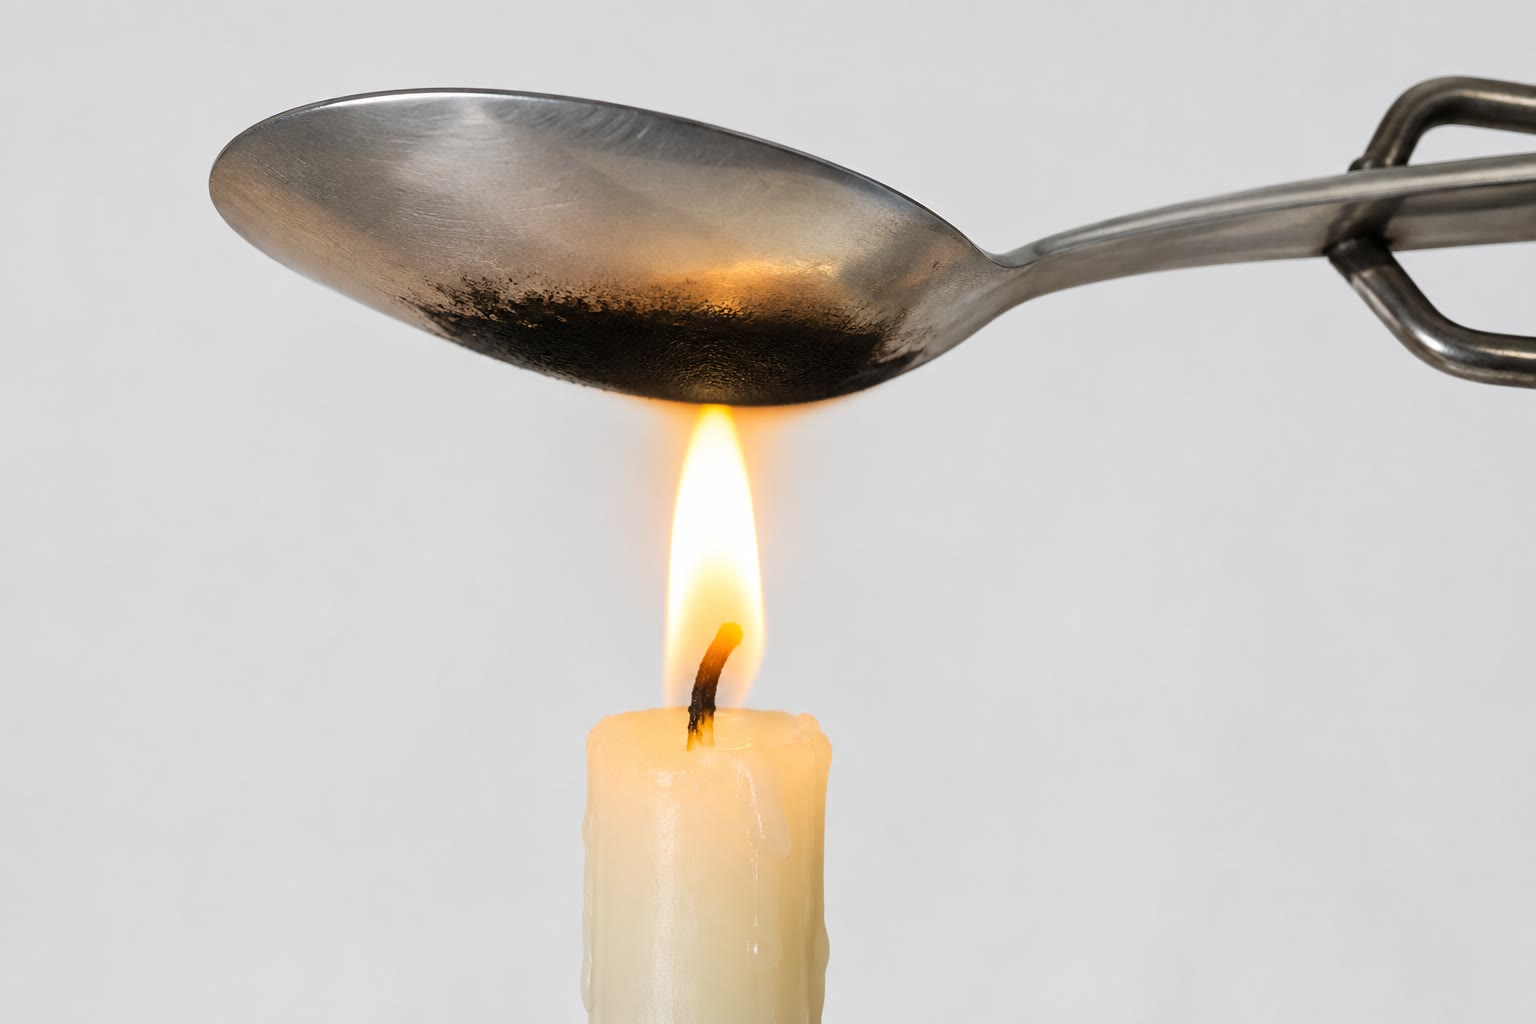
\includegraphics[width=0.45\linewidth]{images/book1/ai/g8-soot-spoon.jpg}

{\small A cold spoon held in a yellow candle flame is blackened by soot:
the \omterm{def:g4:what-a-fire-needs:burning}{combustion} is incomplete.}
\end{omfigure}

\section{Carbon monoxide, a silent danger}

\begin{proposition}[Why carbon monoxide kills]\label{prop:g8:combustion-and-fuels:co}
Carbon monoxide has no colour, no smell and no taste. Breathed in, it
takes the place of oxygen in the blood (the biology book explains how),
causing headaches, sleepiness, and in a closed room unconsciousness and
death. It is made by any \omterm{def:g4:what-a-fire-needs:fuel}{fuel} \omterm{def:g4:what-a-fire-needs:burning}{burning} short of \omterm{def:g4:air-a-mixture-of-gases:air}{air}: a gas boiler or
water heater badly serviced or with a blocked flue, a stove in a closed
tent, a barbecue or a generator used indoors.
\end{proposition}

\begin{safety}{\ghs[0.8cm]{GHS02}\ghs[0.8cm]{GHS04}\ghs[0.8cm]{GHS06}\ghs[0.8cm]{GHS08}}
% ledger: ghs:CO
Carbon monoxide: extremely flammable gas (GHS02), supplied under pressure
(GHS04); toxic if inhaled (GHS06); damages organs by repeated exposure
and may harm the unborn child (GHS08).
\end{safety}

\begin{remark}[Preventing poisoning]\label{rem:g8:combustion-and-fuels:prevent}
Gas appliances are serviced regularly by a professional, flues and \omterm{def:g4:air-a-mixture-of-gases:air}{air}
vents are never blocked, barbecues and generators are used only
outdoors, and a carbon monoxide alarm is fitted near any burner.
\end{remark}

\begin{omfigure}
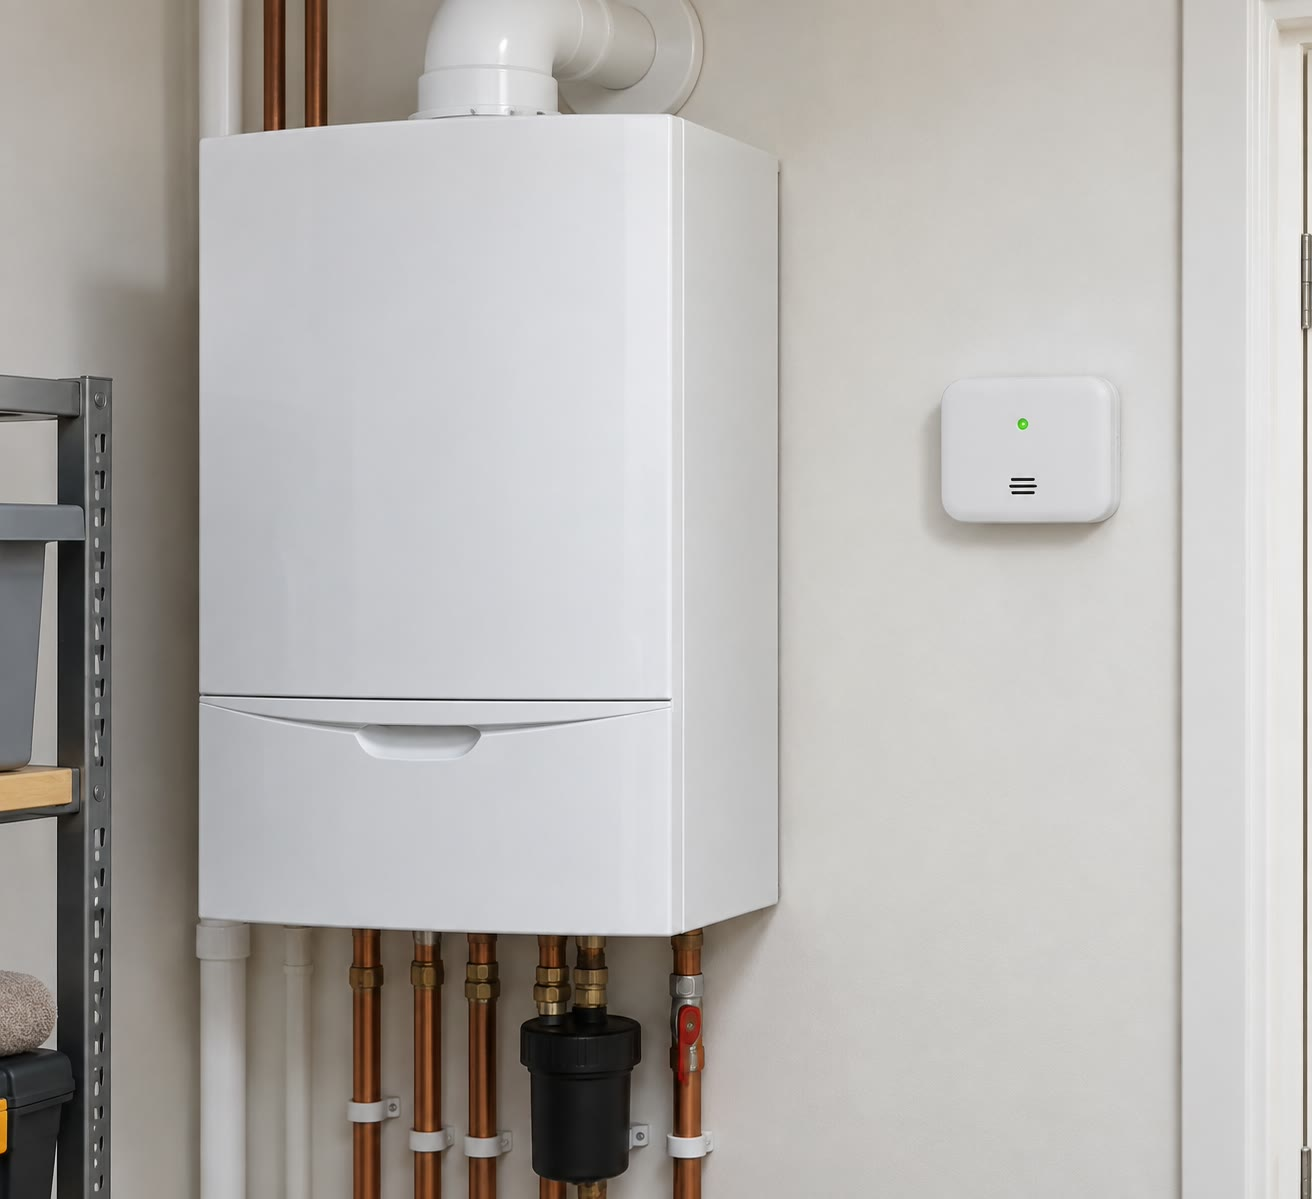
\includegraphics[width=0.45\linewidth]{images/book1/ai/g8-boiler-alarm.jpg}

{\small A gas boiler and, beside it, a carbon monoxide alarm.}
\end{omfigure}

\section{Carbon dioxide and the greenhouse effect}

\begin{definition}[Greenhouse gas]\label{def:g8:combustion-and-fuels:greenhouse}
A \emph{greenhouse gas}\index{greenhouse gas} is a gas of the \omterm{def:g4:air-a-mixture-of-gases:air}{air} that
lets the sunlight through but holds back part of the heat that the
Earth's surface sends back towards space, and so warms the lower
atmosphere. Water vapour, carbon dioxide and methane are greenhouse
gases; nitrogen and oxygen are not. (How this happens is explained in the
physics book.)
\end{definition}

\begin{proposition}[Carbon dioxide in the air is rising]\label{prop:g8:combustion-and-fuels:rising}
% ledger: co2:mlo-1959, co2:mlo-2025 (rise 111.4 ppm, +35 %)
The amount of carbon dioxide in the \omterm{def:g4:air-a-mixture-of-gases:air}{air} has been measured without a
break since 1959 at an observatory on a mountain in the middle of the
Pacific Ocean. It was 316 parts per million (ppm) of \omterm{def:g4:air-a-mixture-of-gases:air}{air} in 1959 and 427
ppm in 2025: a rise of about \qty{35}{\percent} in a human lifetime,
mostly from the \omterm{def:g4:what-a-fire-needs:burning}{burning} of coal, oil and natural gas. The extra carbon
dioxide strengthens the greenhouse effect and warms the climate.
\end{proposition}

\begin{omfigure}
\begin{tikzpicture}
\begin{axis}[width=0.85\linewidth, height=6cm, xmin=1955, xmax=2030,
    ymin=300, ymax=440, xlabel={year}, ylabel={carbon dioxide (ppm)},
    axis lines*=left, ymajorgrids, grid style={gray!20},
    tick label style={font=\small, /pgf/number format/1000 sep={}},
    label style={font=\small}]
\addplot[omDef, thick, mark=*, mark size=0.8pt]
  table[x=year, y=ppm] {figdata/out/grade-8-co2-record.dat};
\node[anchor=west, font=\small] at (axis cs:1962,306) {316 ppm in 1959};
\node[anchor=east, font=\small] at (axis cs:2023,428) {427 ppm in 2025};
\end{axis}
\end{tikzpicture}

{\small Yearly average carbon dioxide in the \omterm{def:g4:air-a-mixture-of-gases:air}{air}, measured since 1959
(NOAA Global Monitoring Laboratory data; before 1974, Scripps
Institution of Oceanography).}
\end{omfigure}

\section{Fossil and renewable fuels}

\begin{definition}[Fossil and renewable fuels]\label{def:g8:combustion-and-fuels:fossil}
A \emph{fossil fuel}\index{fossil fuel} --- coal, oil, natural gas ---
formed underground over millions of years from the remains of ancient
plants and sea creatures. A \emph{renewable fuel}\index{renewable fuel}
is made from plants grown today, or from waste: wood, biogas from
manure and food waste, ethanol made from sugar beet or cane.
\end{definition}

\begin{proposition}[Where the carbon comes from]\label{prop:g8:combustion-and-fuels:cycle}
Plants take carbon dioxide from the \omterm{def:g4:air-a-mixture-of-gases:air}{air} to grow. \omterm{def:g4:what-a-fire-needs:burning}{Burning} a \omterm{def:g8:combustion-and-fuels:fossil}{renewable
fuel} gives back carbon dioxide that its plants took from the \omterm{def:g4:air-a-mixture-of-gases:air}{air} a few
years ago. \omterm{def:g4:what-a-fire-needs:burning}{Burning} a \omterm{def:g8:combustion-and-fuels:fossil}{fossil fuel} releases carbon that was locked away
underground for millions of years: it adds carbon dioxide to the \omterm{def:g4:air-a-mixture-of-gases:air}{air}.
\end{proposition}

\begin{omfigure}
\begin{tikzpicture}[font=\small,
    box/.style={draw=omDef, fill=omDef!6, rounded corners=2pt, align=center,
      minimum height=0.9cm, text width=2.6cm}]
  \node[box] (air) at (0,3) {carbon dioxide\\ in the air};
  \node[box] (plants) at (5.6,3) {plants grow\\ (take \ce{CO2})};
  \node[box] (fuel) at (5.6,0.4) {wood, biogas,\\ bioethanol};
  \node[box, draw=black!50, fill=black!8] (fossil) at (0,0.4) {coal, oil, gas:\\ underground};
  \draw[->, thick, omProp] (air) -- (plants);
  \draw[->, thick, omProp] (plants) -- (fuel);
  \draw[->, thick, omProp] (fuel) -- (air);
  \node[text=black, font=\footnotesize, align=left, anchor=north west] at (1.5,1.45)
    {burning,\\ a few years later};
  \draw[->, thick, black!60] (fossil) -- node[midway, left, text=black, font=\footnotesize,
    align=right] {burning:\\ carbon stored\\ for millions\\ of years} (air);
\end{tikzpicture}

{\small \omterm{def:g8:combustion-and-fuels:fossil}{Renewable fuels} return to the \omterm{def:g4:air-a-mixture-of-gases:air}{air} the carbon their plants took
from it; \omterm{def:g8:combustion-and-fuels:fossil}{fossil fuels} add carbon that had been stored underground.}
\end{omfigure}

\begin{omfigure}
\begin{minipage}[t]{0.48\linewidth}\centering
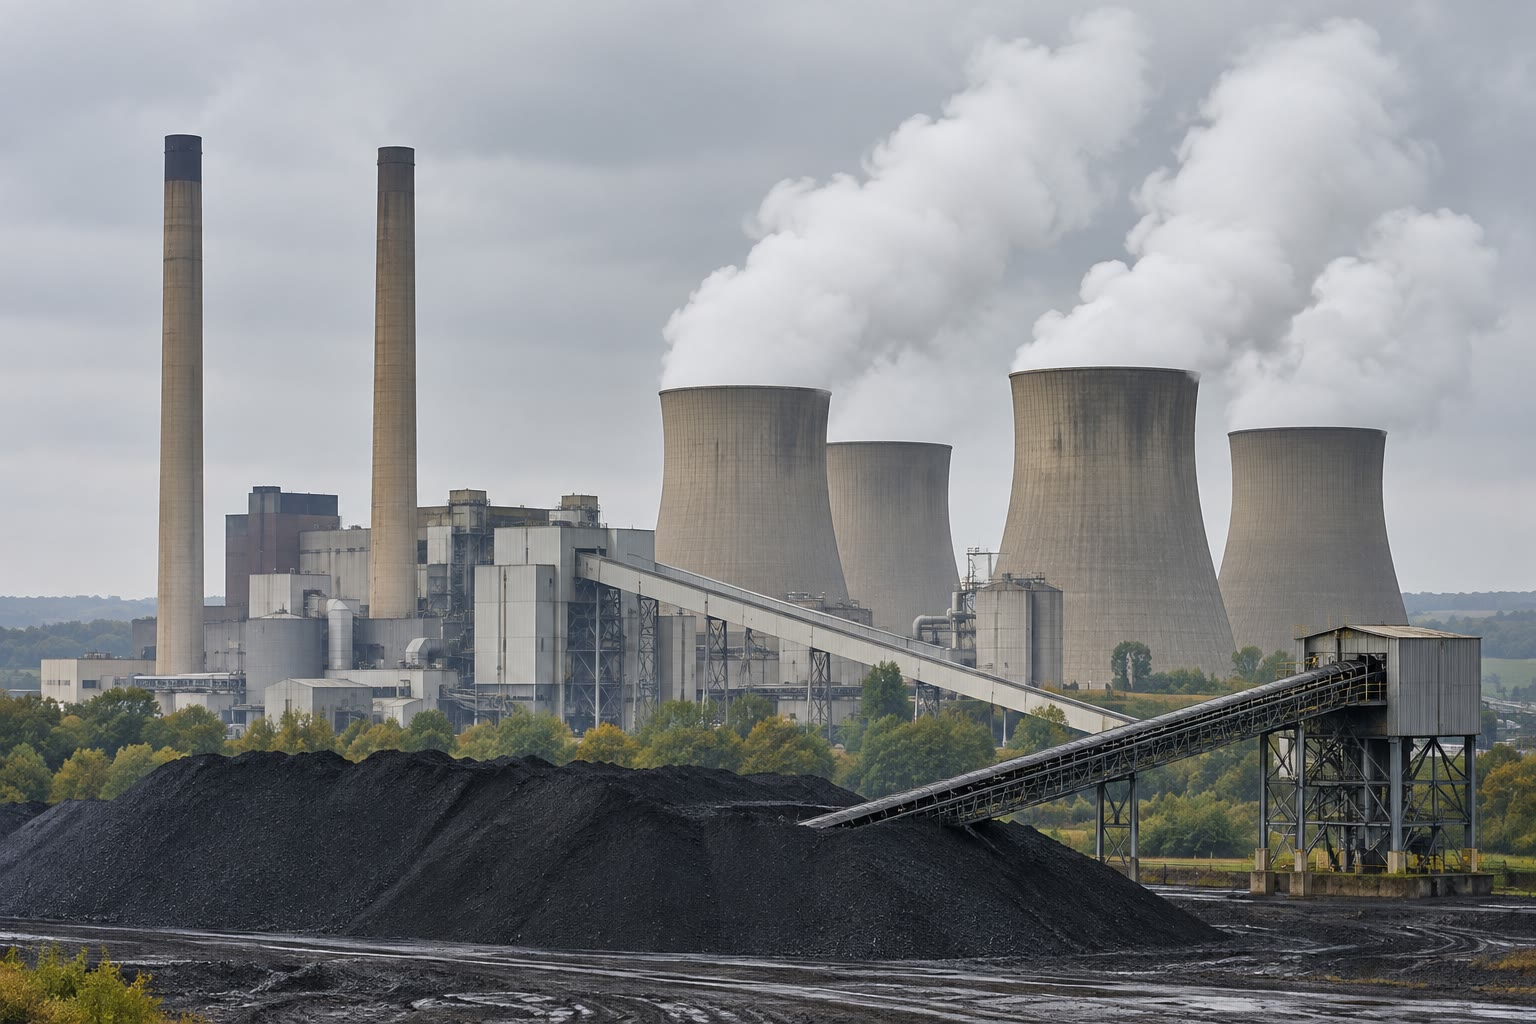
\includegraphics[width=\linewidth,height=4.6cm,keepaspectratio]{images/book1/ai/g8-coal-plant.jpg}

{\small A coal-burning power station.}
\end{minipage}\hfill
\begin{minipage}[t]{0.48\linewidth}\centering
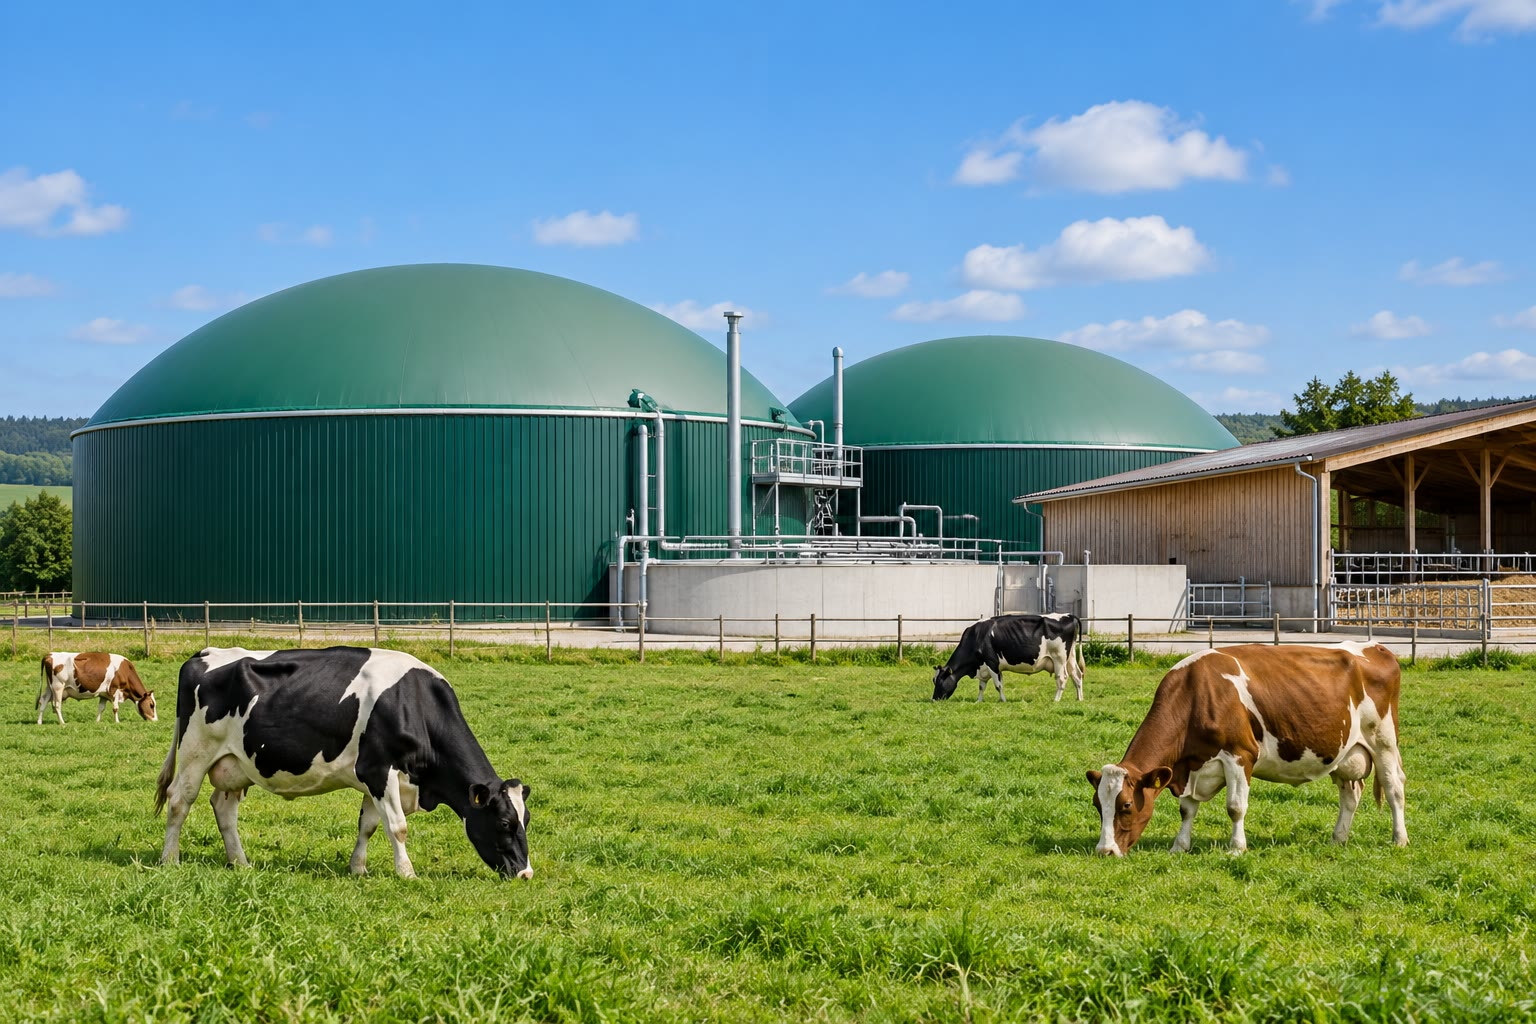
\includegraphics[width=\linewidth,height=4.6cm,keepaspectratio]{images/book1/ai/g8-biogas-farm.jpg}

{\small A farm biogas plant: manure becomes a \omterm{def:g8:combustion-and-fuels:fossil}{renewable fuel}.}
\end{minipage}
\end{omfigure}

\section{Exercises}

\begin{exercise}[$\star$]\label{exo:g8:combustion-and-fuels:1}
Write the \omterm{def:g8:balanced-equations:equation}{balanced equation} of the \omterm{def:g8:combustion-and-fuels:complete}{complete combustion} of carbon.
\end{exercise}

\begin{exercise}[$\star$]\label{exo:g8:combustion-and-fuels:2}
What is the difference between a complete and an \omterm{def:g8:combustion-and-fuels:complete}{incomplete combustion}?
\end{exercise}

\begin{exercise}[$\star$]\label{exo:g8:combustion-and-fuels:3}
Why is carbon monoxide called a silent danger?
\end{exercise}

\begin{exercise}[$\star$]\label{exo:g8:combustion-and-fuels:4}
Fossil or renewable: coal, wood, natural gas, biogas, petrol, ethanol
from sugar beet?
\end{exercise}

\begin{exercise}[$\star\star$]\label{exo:g8:combustion-and-fuels:5}
Write the \omterm{def:g8:balanced-equations:equation}{balanced equation} of the \omterm{def:g8:combustion-and-fuels:complete}{complete combustion} of propane,
\ce{C3H8}.
\end{exercise}

\begin{exercise}[$\star\star$]\label{exo:g8:combustion-and-fuels:6}
Ethanol, \ce{C2H6O}, burns completely in oxygen. Balance
\ce{C2H6O + O2 -> CO2 + H2O}. % ce-unbalanced-ok (to balance)
\end{exercise}

\begin{exercise}[$\star\star$]\label{exo:g8:combustion-and-fuels:7}
A pan held over a yellow flame turns black underneath. What is the black
substance? What does it tell us about the \omterm{def:g4:what-a-fire-needs:burning}{combustion}?
\end{exercise}

\begin{exercise}[$\star\star$]\label{exo:g8:combustion-and-fuels:8}
Read the carbon dioxide curve: about how much carbon dioxide did the \omterm{def:g4:air-a-mixture-of-gases:air}{air}
hold in 1980 and in 2000? By how many ppm did it rise in those twenty
years?
\end{exercise}

\begin{exercise}[$\star\star$]\label{exo:g8:combustion-and-fuels:9}
Why does \omterm{def:g4:what-a-fire-needs:burning}{burning} wood add less carbon dioxide to the \omterm{def:g4:air-a-mixture-of-gases:air}{air}, over the years,
than \omterm{def:g4:what-a-fire-needs:burning}{burning} coal, although both give carbon dioxide?
\end{exercise}

\begin{exercise}[$\star\star$]\label{exo:g8:combustion-and-fuels:10}
Balance the \omterm{def:g8:combustion-and-fuels:complete}{incomplete combustion} of carbon to carbon monoxide,
\ce{C + O2 -> CO}. % ce-unbalanced-ok (to balance)
\end{exercise}

\begin{exercise}[$\star\star\star$]\label{exo:g8:combustion-and-fuels:11}
From 1959 (316 ppm) to 2025 (427 ppm), by what percentage did the
carbon dioxide of the \omterm{def:g4:air-a-mixture-of-gases:air}{air} increase? Round to the nearest whole number.
\end{exercise}

\begin{exercise}[$\star\star\star$]\label{exo:g8:combustion-and-fuels:12}
A gas heater is used in a small room with the window closed. Explain,
using two equations of this chapter, how the \omterm{def:g4:what-a-fire-needs:burning}{combustion} can change from
complete to incomplete as time passes, and why this is dangerous.
\end{exercise}

\section{Problem: The Stove in the Tent}

\begin{problem}[{Weekend problem --- a camping stove, the gas it burns,
what it makes, and why it never goes inside a tent}]
\label{pb:g8:combustion-and-fuels:1}
% ledger: ghs:propane
A camping stove burns propane, \ce{C3H8}, from a cartridge holding
\qty{450}{g} of it. In the open \omterm{def:g4:air-a-mixture-of-gases:air}{air} the flame is blue. Take these mass
proportions, worked out from the \omterm{def:g8:balanced-equations:equation}{balanced equation}: \qty{44}{g} of
propane \omterm{def:g4:what-a-fire-needs:burning}{burning} completely give \qty{132}{g} of carbon dioxide.

\medskip
\noindent\textbf{Part I --- The equations.}
\begin{enumerate}
  \item Write the \omterm{def:g8:balanced-equations:equation}{balanced equation} of the \omterm{def:g8:combustion-and-fuels:complete}{complete combustion} of
        propane.
  \item Check it by counting the \omterm{def:g7:atoms-and-molecules:atom}{atoms} of each kind on each side.
  \item Balance the \omterm{def:g8:combustion-and-fuels:complete}{incomplete combustion}
        \ce{C3H8 + O2 -> CO + H2O}. % ce-unbalanced-ok (to balance)
  \item Which of the two needs more oxygen per propane \omterm{def:g7:atoms-and-molecules:molecule}{molecule}?
\end{enumerate}

\medskip
\noindent\textbf{Part II --- Inside a tent.}
\begin{enumerate}[resume]
  \item A stove lit inside a closed tent soon burns with a yellow flame.
        Explain why.
  \item Which dangerous gas is then formed? Give two of its properties
        that make it hard to notice.
  \item The propane cartridge carries two pictograms. Name them and say
        what each means.
  \item Give two rules for using a camping stove safely.
\end{enumerate}

\medskip
\noindent\textbf{Part III --- The carbon dioxide of one cartridge.}
\begin{enumerate}[resume]
  \item How many times heavier is the carbon dioxide formed than the
        propane burnt?
  \item Where do the extra grams come from?
  \item Is propane a \omterm{def:g8:combustion-and-fuels:fossil}{fossil fuel} or a \omterm{def:g8:combustion-and-fuels:fossil}{renewable fuel}? Does \omterm{def:g4:what-a-fire-needs:burning}{burning} it add
        carbon dioxide to the \omterm{def:g4:air-a-mixture-of-gases:air}{air}?
  \item Compute the mass of carbon dioxide released when a whole
        \qty{450}{g} cartridge burns completely.
\end{enumerate}
\end{problem}
